% Provenance (never printed): see sources/outline_sources.md (Year 1: hotspots and
% mantle plumes; hotspot chains and absolute plate motion; large igneous provinces).
% Hotspot map, pole fit, rates and swell from figdata/bachelor-1/hotspots.py (data
% data/derived/bachelor-1-hotspots.csv, Table 1 of the Morgan and Morgan 2007 electronic
% supplement); exercise and problem values in the Book 3 scratch calculators calc/ch15.py and
% calc/ch15ex.py. "Hotspot" is re-founded from Book 1 (g7 volcanoes), "hotspot track"
% from Book 2 (g11 plate-motions); Book 2 owns the age--distance fit of the Hawaiian
% chain, so this chapter fits the Pacific Euler pole from track directions instead.
\chapter{Points chauds et volcanisme intraplaque}\label{ch:b1:hotspots}

À partir de janvier 1983, et pendant des décennies, le Kilauea, sur l'île d'Hawaï,
est entré en éruption presque sans pause depuis un évent de sa zone de rift est,
Pu\textquoteleft u~\textquoteleft O\textquoteleft o, déversant environ
\qty{0.12}{km^3} de lave par an. Le Kilauea se dresse au milieu de la plaque pacifique,
à des milliers de kilomètres de toute dorsale ou fosse. Au nord-ouest les
îles d'Hawaï sont de plus en plus anciennes, puis elles s'enfoncent sous la mer et la
chaîne se poursuit en une ligne de volcans noyés sur des milliers de kilomètres de plus.
La tectonique des plaques explique les volcans aux limites de plaques~; ce chapitre traite
de ceux qu'elle n'explique pas directement, les \omterm{def:b1:hotspots:hotspot}{points chauds}, et de ce qu'ils nous
apprennent en retour~: comment les plaques se déplacent au-dessus du \omterm{def:b1:layered-earth:layers}{manteau} profond, quelle quantité de chaleur et de roche
monte d'en bas, et comment quelques énormes épanchements de lave, les \omterm{def:b1:hotspots:lip}{grandes
provinces magmatiques}, ont été faits.
% ledger: pp1801:kilauea-rate

\begin{recall}
Un \omterm{def:b1:hotspots:hotspot}{point chaud} alimente des volcans depuis le fond du \omterm{def:b1:layered-earth:layers}{manteau} tandis que la plaque se déplace au-dessus
de lui, et la plaque emporte une \omterm{def:b1:hotspots:track}{trace de point chaud} dont les volcans sont de plus en plus anciens
avec la distance (livre~1, année~7~; livre~2, année~11). Une plaque qui tourne avec le \omterm{def:b1:plate-kinematics:euler-pole}{vecteur d'Euler}
$\vec\omega$ se déplace à $\vec v = \vec\omega\times\vec r$, à la vitesse
$\omega R\sin\Delta$, perpendiculairement au \omterm{def:b1:spherical-astronomy:spherical-triangle}{grand cercle} qui la joint au
pôle (\cref{ch:b1:plate-kinematics})~; le relief est soutenu par l'\omterm{def:b1:isostasy-gravity:isostasy}{isostasie}
(\cref{ch:b1:isostasy-gravity})~; la roche chaude est plus légère de la fraction
$\alpha\,\Delta T$ (\cref{ch:b1:rifts-ridges-margins}).
\end{recall}

\section{Points chauds et panaches mantelliques}\label{sec:b1:hotspots:plumes}

\begin{definition}[Point chaud]\label{def:b1:hotspots:hotspot}
Un \emph{point chaud}\index{point chaud} est une région de volcanisme dont la position ne dépend
pas des limites de plaques, active sur des dizaines de millions d'années,
et que l'on pense alimentée par du \omterm{def:b1:layered-earth:layers}{manteau} plus chaud que le \omterm{def:b1:layered-earth:layers}{manteau} qui l'entoure.
\end{definition}

Combien il y a de \omterm{def:b1:hotspots:hotspot}{points chauds} dépend de ce que l'on compte. Le tableau de \omterm{def:b1:hotspots:hotspot}{points chauds}
utilisé dans ce chapitre en liste 68, mais ses auteurs laissent de côté plusieurs
objets qu'ils jugent ne pas enregistrer le mouvement d'une plaque, et ils n'en tiennent certains
que pour probables. Certains \omterm{def:b1:hotspots:hotspot}{points chauds}, parmi lesquels Hawaï, l'Islande et
la Réunion, ont de longues traces régulières et une grande production, comme en aurait une source
profonde~; d'autres sont petits et de courte durée. La plupart des volcans de \omterm{def:b1:hotspots:hotspot}{points chauds} émettent du basalte~;
là où un \omterm{def:b1:hotspots:hotspot}{point chaud} se trouve sous un continent, le basalte chaud fait fondre la \omterm{def:b1:layered-earth:layers}{croûte}, et
les grandes éruptions tournent à la rhyolite, comme à Yellowstone.
% ledger: mm07:table, data:b3-hotspots, yvo:calderas

\begin{definition}[Panache mantellique]\label{def:b1:hotspots:plume}
Un \emph{panache mantellique}\index{panache mantellique} est une colonne de roche chaude et flottante du \omterm{def:b1:layered-earth:layers}{manteau}
qui monte d'une \omterm{def:b1:heat-budget:boundary-layer}{couche limite thermique} profonde du \omterm{def:b1:layered-earth:layers}{manteau}. Un nouveau panache
a une grosse \emph{tête} bulbeuse sur une longue et étroite \emph{queue}, ou conduit~; une fois
que la tête s'est étalée sous la \omterm{def:b1:layered-earth:lithosphere}{lithosphère}, la queue continue d'alimenter la
surface en magma pendant des dizaines de millions d'années.
\end{definition}

La forme vient du laboratoire. Dans des expériences en cuve des années 1970, une couche
de fluide léger moins visqueux que le fluide au-dessus montait comme une poche ronde alimentée
par un tuyau derrière elle~: un champignon. La tête d'un \omterm{def:b1:hotspots:plume}{panache mantellique} qui atteint la base
de la \omterm{def:b1:layered-earth:lithosphere}{lithosphère} s'étale et s'aplatit~; la pression baisse, et la roche chaude
fond en grande quantité. Les basaltes de trapps cadrent avec ce tableau~: leur volcanisme
dure une dizaine de millions d'années, mais l'essentiel de leur volume est émis en environ un
million d'années ou moins, et ils vont souvent de pair avec la dislocation d'un
continent (\cref{sec:b1:hotspots:lips}).
% ledger: hist:plumes (Whitehead and Luther 1975), cr03:summary

\begin{omfigure}
\begin{tikzpicture}[font=\scriptsize,
  lbl/.style={fill=white, fill opacity=0.8, text opacity=1, inner sep=1pt, align=center}]
% ---- panel (a): the head arrives ----
\begin{scope}
\clip (0,-5) rectangle (6.4,1.3);
\fill[orange!12] (0,-5) rectangle (6.4,0);
\fill[omSea!45] (0,0) rectangle (6.4,0.55);
\fill[omLithBasalt!55] (0,0) rectangle (6.4,-0.9);
% flood basalt: a stack of flat flows on the sea floor
\fill[black!55] (2.5,0) -- (2.7,0.32) -- (6.1,0.32) -- (6.3,0) -- cycle;
\foreach \y in {0.08,0.16,0.24} \draw[white!70!black, line width=0.3pt] (2.62,\y) -- (6.18,\y);
% plume: tail and flattened head
\fill[red!40] (4.25,-5) -- (4.25,-1.7) -- (4.55,-1.7) -- (4.55,-5) -- cycle;
\fill[red!40] (4.4,-1.45) ellipse[x radius=1.9, y radius=0.55];
\draw[red!60!black, line width=0.4pt] (4.25,-5) -- (4.25,-1.95) (4.55,-5) -- (4.55,-1.95);
\draw[red!60!black, line width=0.4pt] (4.4,-1.45) ellipse[x radius=1.9, y radius=0.55];
% melt rising through the plate
\foreach \x in {3.2,3.9,4.6,5.3}
  \draw[red!75!black, line width=0.6pt, decorate, decoration={snake, amplitude=0.6pt, segment length=3pt}] (\x,-1.1) -- (\x,0.05);
\end{scope}
\draw[black!70] (0,-5) rectangle (6.4,1.3);
\node[lbl, anchor=north west] at (0.1,1.25) {(a) la tête arrive};
\node[lbl, anchor=west] at (0.1,-0.45) {lithosphère};
\node[lbl, anchor=west] at (0.1,0.3) {mer};
\node[lbl, anchor=south] at (4.4,0.62) {basalte de trapps (LIP)};
\node[lbl, anchor=east] (ph) at (1.9,-1.75) {tête du panache};
\draw[black!70] (ph.east) -- (2.7,-1.6);
\node[lbl, anchor=east] at (4.1,-3.6) {queue du panache};
\node[lbl, anchor=west] at (0.1,-4.6) {manteau};
% ---- panel (b): the plate has moved on ----
\begin{scope}[xshift=6.8cm]
\begin{scope}
\clip (0,-5) rectangle (6.4,1.3);
\fill[orange!12] (0,-5) rectangle (6.4,0);
\fill[omSea!45] (0,0) rectangle (6.4,0.55);
\fill[omLithBasalt!55] (0,0) rectangle (6.4,-0.9);
% the flood basalt, carried away to the left
\fill[black!55] (-0.9,0) -- (-0.7,0.32) -- (1.0,0.32) -- (1.2,0) -- cycle;
\foreach \y in {0.08,0.16,0.24} \draw[white!70!black, line width=0.3pt] (-0.8,\y) -- (1.08,\y);
% the chain: older volcanoes to the left, lower (they sank as the plate cooled)
\fill[black!35] (1.45,0) -- (1.75,0.2) -- (2.05,0) -- cycle;
\fill[black!38] (2.15,0) -- (2.5,0.3) -- (2.85,0) -- cycle;
\fill[black!42] (2.95,0) -- (3.35,0.42) -- (3.75,0) -- cycle;
\fill[black!65] (3.95,0) -- (4.45,0.95) -- (4.55,0.97) -- (5.05,0) -- cycle;
\fill[red!70!black] (4.43,0.93) -- (4.57,0.95) -- (4.5,1.12) -- cycle;
% the plume tail, still in place, and a small spread of hot rock under the plate
\fill[red!40] (4.35,-5) -- (4.35,-1.1) -- (4.65,-1.1) -- (4.65,-5) -- cycle;
\fill[red!40] (4.5,-1.05) ellipse[x radius=0.75, y radius=0.2];
\draw[red!60!black, line width=0.4pt] (4.35,-5) -- (4.35,-1.2) (4.65,-5) -- (4.65,-1.2);
\draw[red!75!black, line width=0.6pt, decorate, decoration={snake, amplitude=0.6pt, segment length=3pt}] (4.5,-0.95) -- (4.5,0.8);
\end{scope}
\draw[black!70] (0,-5) rectangle (6.4,1.3);
\node[lbl, anchor=north west] at (0.1,1.25) {(b) bien plus tard};
\draw[->, line width=1pt] (3.2,-0.45) -- (1.2,-0.45) node[midway, above=1pt, lbl] {mouvement de la plaque};
\node[lbl, anchor=south] at (0.55,0.38) {la LIP};
\node[lbl, anchor=south] at (2.7,0.62) {plus ancien, éteint};
\node[lbl, anchor=west] at (5.0,0.95) {volcan\\actif};
\node[lbl, anchor=east] at (4.2,-3.6) {queue du panache};
\node[lbl, anchor=west] at (4.75,-2.6) {reste dans\\le manteau};
\end{scope}
\end{tikzpicture}
\par\smallskip{\small Le modèle de panache d'un \omterm{def:b1:hotspots:hotspot}{point chaud} (schématique, hors échelle).
(a)~Un nouveau panache~: sa tête s'aplatit sous la \omterm{def:b1:layered-earth:lithosphere}{lithosphère} et fond en se
décomprimant, et un basalte de trapps, une \omterm{def:b1:hotspots:lip}{grande province magmatique}, est émis en
quelques millions d'années ou moins. (b)~Des dizaines de millions d'années plus tard la plaque a
emporté la province~; l'étroite queue alimente encore un volcan actif, et
les volcans qu'elle a construits avant sont éteints, de plus en plus anciens avec la distance, et plus bas,
car ils s'enfoncent avec la plaque qui se refroidit.}
\label{fig:b1:hotspots:plume}
\end{omfigure}

Quelles sont les preuves des panaches~? D'abord, les chaînes à \omterm{def:b1:hotspots:track}{progression des âges} elles-mêmes,
qu'une source étroite fixe sous une plaque mobile explique d'emblée
(\cref{sec:b1:hotspots:tracks}). Ensuite, les laves de certains \omterm{def:b1:hotspots:hotspot}{points chauds} portent des
rapports inhabituellement élevés de l'isotope léger de l'hélium à l'isotope lourd, lus comme la
signature d'un réservoir profond qui a gardé une part du gaz avec lequel la Terre a été faite.
Troisièmement, les sources sont chaudes~: les laves des îles océaniques et des plateaux indiquent
un \omterm{def:b1:layered-earth:layers}{manteau} plus chaud de 200 à \qty{300}{\celsius} que le \omterm{def:b1:layered-earth:layers}{manteau} sous les dorsales,
dont la température potentielle se situe entre 1280 et \qty{1400}{\celsius}. Quatrièmement,
les images sismiques du \omterm{def:b1:layered-earth:layers}{manteau}~: sous Hawaï, un réseau de sismomètres sur le
fond marin et sur les îles a imagé une colonne chaude descendant dans le \omterm{def:b1:layered-earth:layers}{manteau}
inférieur, et un modèle de tout le \omterm{def:b1:layered-earth:layers}{manteau} construit en 2015 à partir de formes d'onde
sismiques complètes montre de larges colonnes à peu près verticales sous de nombreux grands
\omterm{def:b1:hotspots:hotspot}{points chauds}, montant de la \omterm{def:b1:layered-earth:discontinuity}{limite noyau--manteau} jusqu'à environ \qty{1000}{km} sous
la surface~; sous Hawaï, l'Islande et Samoa elles s'enracinent dans des plaques de
très faible vitesse d'ondes à la base du \omterm{def:b1:layered-earth:layers}{manteau}. La façon dont de telles images sont faites relève
du volume de troisième année.
% ledger: herzberg:tp, wolfe:hawaii, fr15:plumes

Rien de cela n'est une preuve, et le débat est vif. Dans l'hypothèse des plaques,
défendue entre autres par Gillian Foulger et James Natland, le volcanisme de \omterm{def:b1:hotspots:hotspot}{points chauds}
n'est pas particulièrement chaud et n'a pas besoin de panache profond~: c'est un sous-produit de la tectonique
des plaques, alimenté par des sources peu profondes là où la \omterm{def:b1:layered-earth:lithosphere}{lithosphère} est étirée ou
fissurée. Leurs adversaires soutiennent que les preuves en faveur d'au moins quelques panaches profonds
sont solides, bien que les images sismiques ne soient pas encore assez nettes pour trancher~; et
les \omterm{def:b1:hotspots:hotspot}{points chauds}, comme le montre la section suivante, ne sont pas tout à fait fixes.
% ledger: fn03:plate-hypothesis, tarduno:emperor

\section{Traces de points chauds et mouvement des plaques}\label{sec:b1:hotspots:tracks}

\begin{definition}[Trace de point chaud~; progression des âges]\label{def:b1:hotspots:track}
Une \emph{trace de point chaud}\index{trace de point chaud} est la ligne de volcans, de monts sous-marins
et de dorsales volcaniques qu'une plaque emporte loin d'un \omterm{def:b1:hotspots:hotspot}{point chaud} en se déplaçant au-dessus
de lui. Sa \emph{progression des âges}\index{progression des ages@progression des âges} est l'augmentation régulière
des âges de ses volcans avec la distance au volcan actif. La
\emph{direction} d'une trace au \omterm{def:b1:hotspots:hotspot}{point chaud} est l'\omterm{def:b1:spherical-astronomy:horizontal}{azimut}, mesuré depuis le nord,
vers lequel sa partie jeune s'éloigne du \omterm{def:b1:hotspots:hotspot}{point chaud}.
\end{definition}

Si les \omterm{def:b1:hotspots:hotspot}{points chauds} restent fixes dans le \omterm{def:b1:layered-earth:layers}{manteau} profond, une trace enregistre le mouvement de la
plaque au-dessus du \omterm{def:b1:layered-earth:layers}{manteau} profond~: sa direction est celle de la vitesse de la plaque au
\omterm{def:b1:hotspots:hotspot}{point chaud}, et sa \omterm{def:b1:hotspots:track}{progression des âges} donne la vitesse. Le livre~2, année~11, a lu la
vitesse de la plaque pacifique sur les âges des volcans hawaïens. Les
directions seules en disent déjà plus~: elles donnent le \omterm{def:b1:plate-kinematics:euler-pole}{pôle d'Euler}.

\begin{proposition}[Le pôle d'Euler à partir de deux traces]\label{prop:b1:hotspots:two-tracks}
Soit une \omterm{def:b1:plate-kinematics:rigid-plate}{plaque rigide} qui se déplace au-dessus de deux \omterm{def:b1:hotspots:hotspot}{points chauds} fixes aux positions $\vec r_1$ et
$\vec r_2$, et soient $\vec t_1$ et $\vec t_2$ les vecteurs unitaires horizontaux
le long de leurs traces. Si $\vec t_1$ et $\vec t_2$ ne sont pas parallèles, le \omterm{def:b1:plate-kinematics:euler-pole}{vecteur
d'Euler} de la plaque par rapport aux \omterm{def:b1:hotspots:hotspot}{points chauds} est parallèle à
$\vec t_1\times\vec t_2$, et son pôle est le vecteur unitaire
\[
  \vec p = \pm\frac{\vec t_1\times\vec t_2}{\lVert\vec t_1\times\vec t_2\rVert},
\]
avec le signe pour lequel $(\vec p\times\vec r_1)\cdot\vec t_1 > 0$.
\end{proposition}

\begin{proof}
En chaque \omterm{def:b1:hotspots:hotspot}{point chaud} la plaque se déplace avec $\vec v_i = \vec\omega\times\vec r_i$
(\cref{thm:b1:plate-kinematics:velocity}), et la trace pointe le long de lui~:
$\vec v_i = v_i\vec t_i$ avec $v_i > 0$. Un produit vectoriel est perpendiculaire à ses
facteurs, donc $\vec\omega\cdot\vec t_i = 0$ pour $i = 1, 2$~: $\vec\omega$ est
perpendiculaire à deux vecteurs non parallèles, donc parallèle à leur
produit vectoriel. Des deux vecteurs unitaires le long de lui, le pôle est celui autour
duquel la rotation est antihoraire, c'est-à-dire celui pour lequel
$\vec p\times\vec r_1$ pointe dans le sens où la plaque se déplace au premier \omterm{def:b1:hotspots:hotspot}{point chaud},
selon $+\vec t_1$.
\end{proof}

Pour utiliser la proposition il faut, en un point de \omterm{def:b1:spherical-astronomy:geographic}{latitude} $\varphi$ et de \omterm{def:b1:spherical-astronomy:geographic}{longitude}
$\lambda$, les vecteurs unitaires pointant vers l'est et vers le nord,
\[
  \vec e = (-\sin\lambda,\ \cos\lambda,\ 0),\qquad
  \vec n = (-\sin\varphi\cos\lambda,\ -\sin\varphi\sin\lambda,\ \cos\varphi),
\]
dans les axes du \cref{ch:b1:plate-kinematics} ($x$ vers \ang{0}\,N
\ang{0}\,E, $y$ vers \ang{0}\,N \ang{90}\,E, $z$ vers le pôle nord). Une
trace d'\omterm{def:b1:spherical-astronomy:horizontal}{azimut} $\theta$ suit $\vec t = \sin\theta\,\vec e +
\cos\theta\,\vec n$. Avec la trace hawaïenne, d'\omterm{def:b1:spherical-astronomy:horizontal}{azimut} \ang{304}, et la trace
de Louisville, d'\omterm{def:b1:spherical-astronomy:horizontal}{azimut} \ang{316}, la proposition place le pôle de la plaque
pacifique à \ang{56.2}\,S, \ang{124.0}\,E (le problème du week-end fait le
calcul).
% values (hotspots.py): two_pole_lat -56.1805, two_pole_lon 124.008; ledger: data:b3-hotspots

Deux traces déterminent le pôle mais ne peuvent le tester. De nombreuses traces le
surdéterminent, et l'écart dit si les \omterm{def:b1:hotspots:hotspot}{points chauds} se comportent comme un repère fixe. W. Jason
Morgan, qui a proposé les panaches profonds, et Jason Phipps Morgan ont compilé en 2007
un tableau de 68 \omterm{def:b1:hotspots:hotspot}{points chauds}, avec, là où ils pouvaient être mesurées, la direction de
la trace et la vitesse de la plaque au-dessus du \omterm{def:b1:hotspots:hotspot}{point chaud}, chacune avec son
incertitude et un poids pour sa fiabilité~; un \omterm{def:b1:hotspots:hotspot}{point chaud} sous deux plaques, comme
l'Islande, a une ligne pour chacune. Quinze traces pondérées se trouvent sur la plaque
pacifique, treize d'entre elles avec une vitesse.
% ledger: data:b3-hotspots, mm07:table; values (hotspots.py): n_all 71 rows, n_pacific 15, n_rated 13

\begin{method}[Ajuster un pôle d'Euler et une vitesse à des traces de points chauds]\label{met:b1:hotspots:pole-fit}
Soit, pour $N$ \omterm{def:b1:hotspots:hotspot}{points chauds} sur une plaque, les positions, les directions de traces
$\theta_i \pm \sigma_i$ avec des poids $w_i$, et pour certains d'entre eux les vitesses
$v_i$~:
\begin{enumerate}
  \item Pour un pôle d'essai $\vec p$, calculer à chaque \omterm{def:b1:hotspots:hotspot}{point chaud} la direction de
        $\vec p\times\vec r_i$, l'\omterm{def:b1:spherical-astronomy:horizontal}{azimut} $\hat\theta_i$ du mouvement qu'elle
        prédit (\cref{prop:b1:plate-kinematics:speed}).
  \item Former l'écart $S(\vec p) = \sum_i w_i\bigl((\hat\theta_i -
        \theta_i)/\sigma_i\bigr)^2$, chaque différence étant ramenée entre
        \ang{-180} et \ang{180}.
  \item Chercher le pôle qui minimise $S$~: sur une grille de la sphère entière,
        puis sur une grille plus fine autour du meilleur point.
  \item Avec le pôle trouvé, calculer pour chaque \omterm{def:b1:hotspots:hotspot}{point chaud} avec une vitesse sa distance
        angulaire $\Delta_i$ au pôle et $x_i = R\sin\Delta_i$. Les vitesses
        devraient être $v_i = \omega x_i$~: la vitesse des moindres carrés est
        \[
          \omega = \frac{\sum_i x_i v_i}{\sum_i x_i^2},
        \]
        puisque $\frac{\mathrm d}{\mathrm d\omega}\sum_i (v_i - \omega x_i)^2 =
        -2\sum_i x_i(v_i - \omega x_i)$ s'y annule.
  \item Juger l'ajustement~: si les \omterm{def:b1:hotspots:hotspot}{points chauds} étaient fixes et les incertitudes
        honnêtes, $S$ serait proche du nombre de directions moins deux (les
        deux coordonnées du pôle ajusté).
\end{enumerate}
\end{method}

Pour les quinze traces du Pacifique la méthode donne le pôle \ang{63.8}\,S,
\ang{112.5}\,E, à environ \ang{10} du pôle à deux traces, et à partir des treize
vitesses la vitesse $\omega = \qty{0.92}{\degree\per\Ma}$. À Hawaï, à \ang{108.0}
du pôle, l'ajustement prédit un mouvement vers \ang{298} à
\qty{97}{mm.an^{-1}}~; Morgan et Morgan donnent $\ang{304}\pm\ang{3}$ et
\qty[uncertainty-mode=separate]{92 \pm 3}{mm.an^{-1}}. L'écart $S$ vaut 39
là où des \omterm{def:b1:hotspots:hotspot}{points chauds} fixes avec des incertitudes honnêtes donneraient environ 13, et les
vitesses se dispersent autour de la droite de \qty{16}{mm.an^{-1}} (écart quadratique moyen)~: les
\omterm{def:b1:hotspots:hotspot}{points chauds} du Pacifique forment un repère bon à quelques degrés et quelques
centimètres par an près, pas mieux.
% values (hotspots.py): pole_lon 112.48, pole_lat -63.78, chi2 38.7829, omega_deg_myr 0.920609,
% hawaii_delta 107.998, hawaii_pred_az 297.656, hawaii_pred_rate 97.3581, rms_rate 15.966;
% angle between the two poles 9.5 deg (calc/ch15.py); ledger: data:b3-hotspots

Le meilleur test du repère fixe est le coude de la chaîne Hawaï--Empereur.
Le tronçon hawaïen va vers le nord-ouest~; les monts de l'Empereur vont presque
vers le nord, jusqu'au Meiji Guyot, âgé de plus de 81 millions d'années, qui est sur le point de
plonger à la jonction des fosses Kouriles--Kamtchatka et des Aléoutiennes. Le
coude fut-il un changement du mouvement de la plaque~? L'aimantation des laves
de l'Empereur, mesurée sur des carottes forées dans les monts sous-marins, enregistre la \omterm{def:b1:spherical-astronomy:geographic}{latitude} à laquelle
chacune s'est refroidie (la méthode relève du volume de troisième année)~: elles se sont formées
plus au nord qu'Hawaï aujourd'hui, et entre 81 et 47 millions d'années, le
\omterm{def:b1:hotspots:hotspot}{point chaud} lui-même s'est déplacé vers le sud à plus de \qty{40}{mm} par an.
Une bonne part de la chaîne de l'Empereur enregistre le \omterm{def:b1:hotspots:hotspot}{point chaud}, pas la plaque. Pourtant la plaque a changé aussi~:
de nouveaux âges placent le début du coude près du mont sous-marin Kimmei, il y a environ 50 millions
d'années, quand les dorsales d'expansion du Pacifique ont été réorientées. Le panache
peut même être plus ancien que la chaîne~: la tête qui l'a alimenté en premier est censée
avoir fait un plateau il y a environ 100 millions d'années, qui a plongé dans une fosse il y a 20
à 30 millions d'années et se trouve maintenant à environ \qty{810}{km} de profondeur sous
la Sibérie, à l'ouest de la mer d'Okhotsk.
% ledger: tarduno:emperor, sharp:bend, wei:plume-head

\begin{omfigure}
\begin{tikzpicture}
\begin{axis}[omrecord, width=0.78\linewidth, height=6.2cm, xmin=0, xmax=7000, ymin=0, ymax=160,
  xlabel={$R\sin\Delta$, distance à l'axe de rotation (\unit{km})},
  ylabel={vitesse au-dessus du point chaud (\unit{mm.an^{-1}})},
  xticklabel style={/pgf/number format/set thousands separator={}},
  legend style={font=\scriptsize, at={(0.03,0.97)}, anchor=north west, cells={anchor=west}}]
% computed in figdata/bachelor-1/hotspots.py; ledger: data:b3-hotspots; values: omega_deg_myr 0.920609
\addplot[only marks, mark=*, mark size=1.5pt, omDef, error bars/.cd, y dir=both, y explicit]
  table[x=x, y=rate, y error=srate] {figdata/out/bachelor-1-hotspots-rates.dat};
\addlegendentry{points chauds du Pacifique}
\addplot[black, densely dashed, line width=0.7pt] table[x=x, y=rate] {figdata/out/bachelor-1-hotspots-rates-fit.dat};
\addlegendentry{$\omega R\sin\Delta$, $\omega = \ang{0.92}$ par million d'années}
\draw[black!60] (axis cs:6060,90) -- (axis cs:6550,55) node[font=\scriptsize, anchor=north, black] {Hawaï};
\node[font=\scriptsize, anchor=north west] at (axis cs:4880,64) {Louisville};
\node[font=\scriptsize, anchor=west] at (axis cs:3960,43) {Cobb};
\node[font=\scriptsize, anchor=east] at (axis cs:3570,40) {Bowie};
\end{axis}
\end{tikzpicture}
\par\smallskip{\small Les vitesses de la plaque pacifique au-dessus de treize de ses
\omterm{def:b1:hotspots:hotspot}{points chauds}, avec leurs incertitudes, en fonction de la distance de chaque \omterm{def:b1:hotspots:hotspot}{point chaud} à
l'axe de rotation passant par le pôle ajusté. Une \omterm{def:b1:plate-kinematics:rigid-plate}{plaque rigide} tournant autour de ce
pôle les met sur une droite passant par l'origine~; la droite des moindres carrés donne
$\omega = \qty{0.92}{\degree\per\Ma}$. La plupart des \omterm{def:b1:hotspots:hotspot}{points chauds} sont à 6000 à
\qty{6400}{km} de l'axe, où la vitesse est presque la même~; la dispersion
y est plus grande que les barres d'erreur, ce qui montre les limites d'un repère fixe. Données~:
W.~J. et J.~P. Morgan (2007), tableau~1 de leur supplément électronique.}
\label{fig:b1:hotspots:rates}
\end{omfigure}

\begin{omfigure}
\begin{tikzpicture}
\begin{axis}[ommap, width=0.96\linewidth, xtick={-180,-90,...,180}, ytick={-60,0,60},
  legend style={font=\scriptsize, at={(0.01,0.02)}, anchor=south west, cells={anchor=west}}]
% computed in figdata/bachelor-1/hotspots.py; ledger: data:b3-hotspots, data:ne-land, data:pb2002
\addplot[fill=omLithAlluv, draw=black!45, line width=0.2pt, forget plot] table {figdata/out/shared-geo-land.dat};
\addplot[omRidge, line width=0.5pt, forget plot] table {figdata/out/shared-geo-ridge.dat};
\addplot[omRidge!70!black, line width=0.5pt, forget plot] table {figdata/out/shared-geo-transform.dat};
\addplot[omTrench, line width=0.5pt, forget plot] table {figdata/out/shared-geo-subduction.dat};
\addplot[black!65, line width=0.5pt, forget plot] table {figdata/out/shared-geo-collision.dat};
\addplot[black, line width=0.7pt, -{Stealth[length=3.5pt]}, quiver={u=\thisrow{dx}, v=\thisrow{dy}}, forget plot]
  table[x=lon, y=lat] {figdata/out/bachelor-1-hotspots-map-arrows.dat};
\addplot[only marks, mark=*, mark size=1.3pt, draw=black, fill=orange!90!red] table {figdata/out/bachelor-1-hotspots-map-hs.dat};
\addlegendentry{point chaud}
\addplot[only marks, mark=star, mark size=3.2pt, line width=0.8pt, omDef] table {figdata/out/bachelor-1-hotspots-map-pole.dat};
\addlegendentry{pôle d'Euler de la plaque pacifique}
\draw[black, line width=0.7pt, -{Stealth[length=3.5pt]}] (axis cs:-40,-80) -- (axis cs:-25,-80);
\node[font=\scriptsize, anchor=west, fill=white, fill opacity=0.75, text opacity=1, inner sep=1pt]
  at (axis cs:-23,-80) {\qty{10}{cm} par an};
\node[font=\scriptsize, anchor=north, fill=white, fill opacity=0.75, text opacity=1, inner sep=1pt] at (axis cs:-150,16) {Hawaï};
\node[font=\scriptsize, anchor=north, fill=white, fill opacity=0.75, text opacity=1, inner sep=1pt] at (axis cs:-140.6,-56) {Louisville};
\node[font=\scriptsize, anchor=south, fill=white, fill opacity=0.75, text opacity=1, inner sep=1pt] at (axis cs:-100,49) {Yellowstone};
\node[font=\scriptsize, anchor=south, fill=white, fill opacity=0.75, text opacity=1, inner sep=1pt] at (axis cs:-17.3,66) {Islande};
\node[font=\scriptsize, anchor=north, fill=white, fill opacity=0.75, text opacity=1, inner sep=1pt] at (axis cs:55.7,-23.5) {Réunion};
\end{axis}
\end{tikzpicture}
\par\smallskip{\small Les 68 \omterm{def:b1:hotspots:hotspot}{points chauds} de W.~J. et J.~P. Morgan (2007). Flèches~:
le mouvement de la plaque au-dessus de chaque \omterm{def:b1:hotspots:hotspot}{point chaud} là où il a été mesuré, selon la
direction de la trace et avec une longueur proportionnelle à la vitesse (échelle en
bas, au sud de l'Atlantique)~; là où un \omterm{def:b1:hotspots:hotspot}{point chaud} est sous deux plaques, comme l'Islande, les deux sont
dessinées. L'étoile est le \omterm{def:b1:plate-kinematics:euler-pole}{pôle d'Euler} de la plaque pacifique par rapport aux
\omterm{def:b1:hotspots:hotspot}{points chauds}, ajusté aux quinze traces du Pacifique par la
\cref{met:b1:hotspots:pole-fit}~: les flèches du Pacifique tournent autour de lui. Limites de plaques~:
PB2002 (rouge~: dorsales~; rouge foncé~: transformantes~; bleu~: zones de subduction~;
gris~: zones de collision).}
\label{fig:b1:hotspots:map}
\end{omfigure}


Les \omterm{def:b1:hotspots:track}{traces de points chauds} traversent aussi les continents. Quand la plaque nord-américaine s'est déplacée
vers le sud-ouest au-dessus du \omterm{def:b1:hotspots:hotspot}{point chaud} de Yellowstone, une chaîne de grandes caldeiras s'est formée,
de plus en plus anciennes vers le sud-ouest le long de la plaine de la Snake River. À son
extrémité, à la frontière du Nevada et de l'Oregon, la caldeira de McDermitt, large d'environ
\qty{40}{km}, s'est effondrée il y a 16.4 millions d'années lors d'une éruption d'environ
\qty{1000}{km^3}. À Yellowstone même, la première des trois éruptions formant des caldeiras,
il y a 2.1 millions d'années, a libéré quelque \qty{2400}{km^3} de magma et
laissé une caldeira de plus de \qty{100}{km} de large~; la dernière, il y a 640\,000 ans,
a fait l'actuelle caldeira de Yellowstone, de \qty{55}{km} sur 80. Depuis 10 millions
d'années le début des éruptions de caldeiras s'est déplacé vers le nord-est à
$\qty[uncertainty-mode=separate]{2.9 \pm 0.5}{cm}$ par an, et Morgan et
Morgan donnent à la plaque une vitesse de
\qty[uncertainty-mode=separate]{26 \pm 5}{mm.an^{-1}} au-dessus du \omterm{def:b1:hotspots:hotspot}{point chaud}, vers
\ang{235}~; les caldeiras plus anciennes, comme le montre l'\cref{exo:b1:hotspots:8}, se sont déplacées
plus vite.
% ledger: henry:mcdermitt, yvo:calderas, pm90:track, data:b3-hotspots

\section{Renflements, flottabilité et apport de magma}\label{sec:b1:hotspots:swells}

Hawaï ne se dresse pas sur un plancher océanique ordinaire. En 1953 Robert Dietz et
William Menard ont décrit le large soulèvement du fond marin sur lequel reposent les îles,
le renflement hawaïen. Le renflement n'est pas compensé par une \omterm{def:b1:layered-earth:layers}{croûte} épaisse~: il est
soutenu par en dessous par la roche chaude et légère du panache qui s'étale sous
la plaque, un soutien \emph{dynamique}. Sur le renflement le flux de chaleur en
surface est au plus de 5 à \qty{10}{mW.m^{-2}} plus élevé qu'alentour, et peut-être
pas plus élevé du tout.
% ledger: hist:plumes (Dietz and Menard 1953), vh89:swell-heat

Sa forme peut se lire sur la grille mondiale des profondeurs. Prenons des coupes à travers la
trace, perpendiculaires à sa direction, tous les \qty{50}{km} depuis le \omterm{def:b1:hotspots:hotspot}{point chaud} jusqu'à
\qty{1000}{km} en aval~; à chaque distance de l'axe de la chaîne, la
médiane des profondeurs sur ces coupes donne un profil qui garde le renflement et
lisse les volcans isolés (la figure après la prochaine proposition). Loin de la chaîne, à 1000 à
\qty{1500}{km} de part et d'autre, le plancher se trouve à \qty{5274}{m}. Près d'elle,
les îles et monts sous-marins se dressent jusqu'à \qty{3}{km} plus haut~; remplaçons-les par une
droite sur les \qty{300}{km} de la chaîne, et ce qui reste est le
renflement~: haut d'environ \qty{690}{m} au plus, large de quelques centaines de kilomètres de chaque
côté, avec une section de $A \approx \qty{4.8e8}{m^2}$ au-dessus du plancher
éloigné.
% values (hotspots.py): swell_ref -5273.64, swell_height 690.636, swell_area_m2 4.82786e8;
% ledger: data:etopo1, data:b3-hotspots (Hawaii 19.0 N 155.2 W, track 304)

Le renflement mesure le panache. Il est emporté avec la plaque et refait
au-dessus du \omterm{def:b1:hotspots:hotspot}{point chaud}, donc le panache doit fournir de la flottabilité aussi vite que la plaque
l'emporte.

\begin{proposition}[Flux de flottabilité d'un panache]\label{prop:b1:hotspots:buoyancy}
Soit une plaque qui se déplace à la vitesse $v$ au-dessus d'un \omterm{def:b1:hotspots:hotspot}{point chaud}, et soit le renflement autour de
la trace de section $A$ au-dessus du plancher loin d'elle, le renflement étant en
équilibre isostatique (\cref{def:b1:isostasy-gravity:isostasy}) et soutenu
par de la roche légère emportée avec la plaque. Alors le panache livre un déficit
de masse, son \emph{flux de flottabilité}, au taux
\[
  B = (\rho_m - \rho_w)\,A\,v ,
\]
où $\rho_m$ est la masse volumique du \omterm{def:b1:layered-earth:layers}{manteau} et $\rho_w$ celle de l'eau de mer.
\end{proposition}

\begin{proof}
Considérons une colonne à travers le renflement, où le plancher est surélevé de $h$, et une
colonne loin de lui, toutes deux jusqu'à une \omterm{def:b1:isostasy-gravity:isostasy}{profondeur de compensation}. Entre les deux planchers
la colonne éloignée contient de l'eau et la colonne du renflement de la roche~: la colonne du renflement a la
masse supplémentaire $(\rho_m - \rho_w)h$ par unité d'aire là. L'égalité des masses au-dessus de la
\omterm{def:b1:isostasy-gravity:isostasy}{profondeur de compensation} (\cref{prop:b1:isostasy-gravity:equal-mass}) exige un
déficit de masse de même taille plus bas dans la colonne du renflement, dans la roche
légère du panache. À travers la trace, le déficit par unité de longueur de trace est
$\int(\rho_m - \rho_w)h\,\mathrm dy = (\rho_m - \rho_w)A$. En un temps
$\mathrm dt$ la plaque emporte une longueur $v\,\mathrm dt$ de renflement en aval,
avec son déficit, et le renflement au-dessus du \omterm{def:b1:hotspots:hotspot}{point chaud} garde sa forme~: le panache
doit fournir le déficit $(\rho_m - \rho_w)A\,v\,\mathrm dt$.
\end{proof}

\begin{omfigure}
\begin{tikzpicture}
\begin{axis}[omrecord, width=0.86\linewidth, height=6cm, xmin=-1500, xmax=1500, xtick={-1500,-1000,...,1500}, ymin=-6000, ymax=-1000,
  xlabel={distance à travers la chaîne hawaïenne, du sud-ouest au nord-est (\unit{km})},
  ylabel={profondeur du fond marin (\unit{m})},
  xticklabel style={/pgf/number format/set thousands separator={}},
  yticklabel style={/pgf/number format/set thousands separator={}},
  legend style={font=\scriptsize, at={(0.99,0.97)}, anchor=north east, cells={anchor=west}}]
% computed in figdata/bachelor-1/hotspots.py; ledger: data:etopo1, data:b3-hotspots
\addplot[name path=hi, draw=none, forget plot] table[x=d, y=q75] {figdata/out/bachelor-1-hotspots-swell.dat};
\addplot[name path=lo, draw=none, forget plot] table[x=d, y=q25] {figdata/out/bachelor-1-hotspots-swell.dat};
\addplot[omSea!60, forget plot] fill between[of=hi and lo];
\addplot[black, line width=0.8pt] table[x=d, y=med] {figdata/out/bachelor-1-hotspots-swell.dat};
\addlegendentry{profondeur médiane}
\addplot[omDef, line width=0.9pt, densely dashed] table[x=d, y=swell] {figdata/out/bachelor-1-hotspots-swell-ref.dat};
\addlegendentry{renflement, chaîne retirée}
\addplot[black!60, densely dotted, line width=0.7pt] table[x=d, y=ref] {figdata/out/bachelor-1-hotspots-swell-ref.dat};
\addlegendentry{référence, à 1000 à \qty{1500}{km}}
\node[font=\scriptsize, anchor=south] at (axis cs:-330,-3300) {la chaîne};
\end{axis}
\end{tikzpicture}
\par\smallskip{\small Le renflement hawaïen. Chaque point est la médiane de 21 profondeurs,
prises sur des coupes à travers la chaîne tous les \qty{50}{km} depuis le \omterm{def:b1:hotspots:hotspot}{point chaud} jusqu'à
\qty{1000}{km} en aval, à la même distance de l'axe de la chaîne~;
la bande grisée contient la moitié centrale des 21 profondeurs. La chaîne elle-même, une
pointe étroite, est remplacée par une droite (en tirets) pour laisser le renflement, d'environ
\qty{690}{m} au-dessus du plancher loin de la chaîne (en pointillés). Profondeurs~: ETOPO1,
échantillonné à un degré.}
\label{fig:b1:hotspots:swell}
\end{omfigure}

Un flux de flottabilité est un écoulement de masse manquante~: il compte la vitesse à laquelle le panache amène
de la roche légère. Ce qui rend la roche légère est la chaleur, donc le flux de flottabilité est aussi
un flux de chaleur.

\begin{proposition}[Chaleur portée par un panache]\label{prop:b1:hotspots:heat}
Si la roche d'un panache est plus chaude de $\Delta T$ que le \omterm{def:b1:layered-earth:layers}{manteau} qui l'entoure, avec
le coefficient de dilatation thermique $\alpha$ et la capacité thermique massique
$c_p$, son flux de flottabilité $B$ et la chaleur excédentaire qu'il porte, $Q$, vérifient
\[
  Q = \frac{c_p}{\alpha}\,B ,
\]
quel que soit $\Delta T$.
\end{proposition}

\begin{proof}
Soit $\Phi$ la masse de roche chaude que le panache porte par unité de temps. Chaque unité
de volume en est plus légère que le \omterm{def:b1:layered-earth:layers}{manteau} de $\rho_m\alpha\,\Delta T$, ce qui est,
au premier ordre, un déficit de masse $\alpha\,\Delta T$ par unité de masse~: $B =
\alpha\,\Delta T\,\Phi$. Chaque unité de masse porte la chaleur excédentaire
$c_p\,\Delta T$~: $Q = c_p\,\Delta T\,\Phi$. En divisant, $\Delta T$ et $\Phi$
s'éliminent.
\end{proof}

Pour Hawaï, avec $\rho_m - \rho_w = \qty{2300}{kg.m^{-3}}$, $A =
\qty{4.83e8}{m^2}$ et $v = \qty{92}{mm.\year^{-1}} = \qty{2.92e-9}{m.s^{-1}}$,
\[
  B = 2300\times\num{4.83e8}\times\num{2.92e-9} \approx \qty{3240}{kg.s^{-1}}:
\]
le panache amène environ trois tonnes de masse manquante chaque seconde. Les roches
stockent 2 à \qty{3}{MJ} par mètre cube et par kelvin~; avec \qty{3}{MJ} le
\omterm{def:b1:layered-earth:layers}{manteau}, de masse volumique \qty{3300}{kg.m^{-3}}, a
$c_p \approx \qty{910}{J.kg^{-1}.K^{-1}}$~;
avec $\alpha = \qty{3.2e-5}{K^{-1}}$,
\[
  Q = \frac{910}{\num{3.2e-5}}\times3240 \approx \qty{9.2e10}{W},
\]
\qty{0.2}{\percent} des \qty{47}{TW} qui quittent la Terre entière. Le
plus puissant panache de la Terre est un petit poste du bilan thermique de la planète
(\cref{ch:b1:heat-budget})~; l'essentiel de la chaleur s'échappe par le plancher océanique
fait aux dorsales.
% values (hotspots.py): swell_B_kg_s 3237.18; Q = 9.1951e10 W (calc/ch15.py);
% ledger: data:b3-hotspots (92 mm/yr), delaney86:properties (Book 2 row), parsons:plate-model (alpha), dd10:total

Le magma raconte la même histoire. Depuis 81 millions d'années le \omterm{def:b1:hotspots:hotspot}{point chaud} a
construit la chaîne Hawaï--Empereur, environ deux millions de kilomètres cubes de
basalte une fois compté l'enfoncement de la plaque sous sa charge, soit en moyenne
\qty{0.025}{km^3} par an~; mais environ un quart en a été émis durant les six derniers
millions d'années, et le Kilauea seul est alimenté aujourd'hui par environ \qty{0.1}{km^3}
de magma par an. Le Mauna Loa, le plus grand volcan des îles, contient quelque
\qty{74000}{km^3}, et le Mauna Kea, son voisin, s'élève à \qty{4205}{m} au-dessus de
la mer. Pourtant les dorsales font environ \qty{21}{km^3} de \omterm{def:b1:rifts-ridges-margins:oceanic-crust}{croûte océanique} par an, deux
cents fois l'apport actuel du Kilauea.
% ledger: pp1801:chain-volume, pp1801:kilauea-supply, pp1801:volumes, data:pb2002 (ridge_budget.py 21.36 km3/yr)

\begin{omfigure}
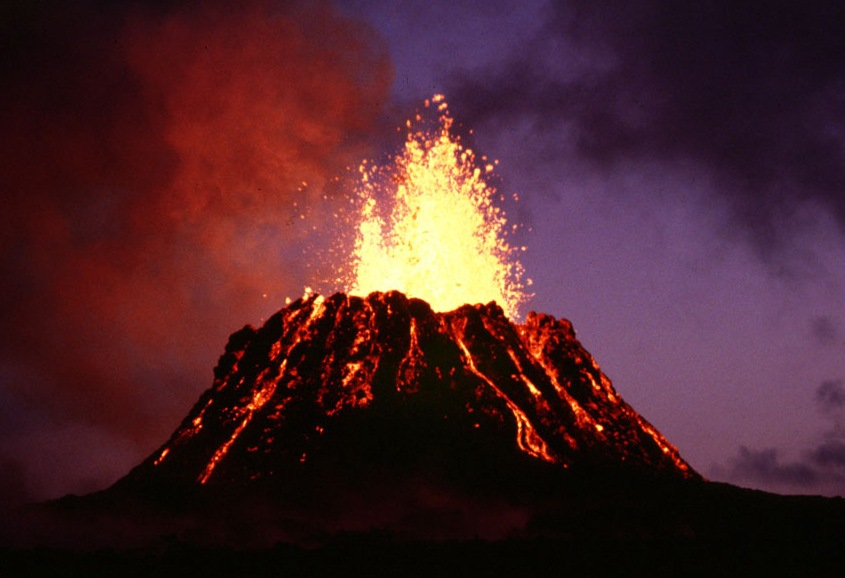
\includegraphics[width=0.55\linewidth]{images/book3/b1-puu-oo-1983.jpg}
\par\smallskip{\small Une fontaine de lave sur le cône Pu\textquoteleft
u~\textquoteleft O\textquoteleft o, sur la zone de rift est du Kilauea,
le 29 juin 1983, durant la première année d'une éruption qui a duré des décennies~:
lave basaltique, chaude et fluide, projetée en un jet et retombant autour de
l'évent. Photographie~: G.~E.~Ulrich, U.S. Geological Survey, domaine public
(Wikimedia Commons).}
\label{fig:b1:hotspots:puu-oo}
\end{omfigure}
% ledger: commons:puu-oo, pp1801:kilauea-rate

\begin{history}[Un repère fixe pour les plaques]
En 1963 John Tuzo Wilson a expliqué les îles hawaïennes, de plus en plus anciennes le long
d'une ligne, par une source de lave tenue dans le cœur lent d'une cellule de convection du \omterm{def:b1:layered-earth:layers}{manteau},
tandis que la partie supérieure plus rapide de la cellule emportait le plancher océanique au-dessus d'elle.
En 1971 et 1972 W. Jason Morgan a fait de cette source un panache, d'environ
\qty{150}{km} de large, montant de la partie la plus basse du \omterm{def:b1:layered-earth:layers}{manteau} et donc presque
fixe tandis que les plaques se déplacent au-dessus de lui~; des expériences en cuve ont vite montré à quoi ressemble un tel
panache. Les \omterm{def:b1:hotspots:hotspot}{points chauds} sont devenus un repère dans lequel les plaques pouvaient être
mesurées par rapport au \omterm{def:b1:layered-earth:layers}{manteau}, et pas seulement les unes par rapport aux autres. Un demi-siècle
plus tard on sait que le repère dérive, le \omterm{def:b1:hotspots:hotspot}{point chaud} d'Hawaï entre autres, mais
assez lentement pour que les traces du Pacifique donnent encore le mouvement de la plaque au-dessus
du \omterm{def:b1:layered-earth:layers}{manteau} à quelques degrés et quelques centimètres par an près, comme l'a montré l'ajustement de ce
chapitre.
\end{history}
% ledger: hist:plumes, tarduno:emperor

\section{Les grandes provinces magmatiques}\label{sec:b1:hotspots:lips}

\begin{definition}[Grande province magmatique]\label{def:b1:hotspots:lip}
Une \emph{grande province magmatique}\index{grande province magmatique} (LIP) est une
accumulation de roche ignée, surtout du basalte, qui n'est pas faite par l'expansion
ordinaire à une dorsale, couvre plus de \qty{e5}{km^2}, contient plus de
\qty{e5}{km^3}, et a été mise en place en au plus environ 50 millions d'années, la plus grande part
en pulsations de 1 à 5 millions d'années qui portent plus des trois quarts de
son volume. Sur terre les LIP sont surtout des basaltes de trapps~; dans les océans, des
plateaux océaniques.
\end{definition}

Une LIP typique couvre environ un million de kilomètres carrés et contient environ un
million de kilomètres cubes de lave, la plus grande part émise en environ un million d'années
ou moins. Leurs laves sont empilées en coulées presque horizontales, que l'érosion découpe en
marches, les \emph{trapps} de leurs noms. Le tableau liste les principales des
260 derniers millions d'années.
% ledger: be08:definition, cr03:summary

\begin{omfigure}
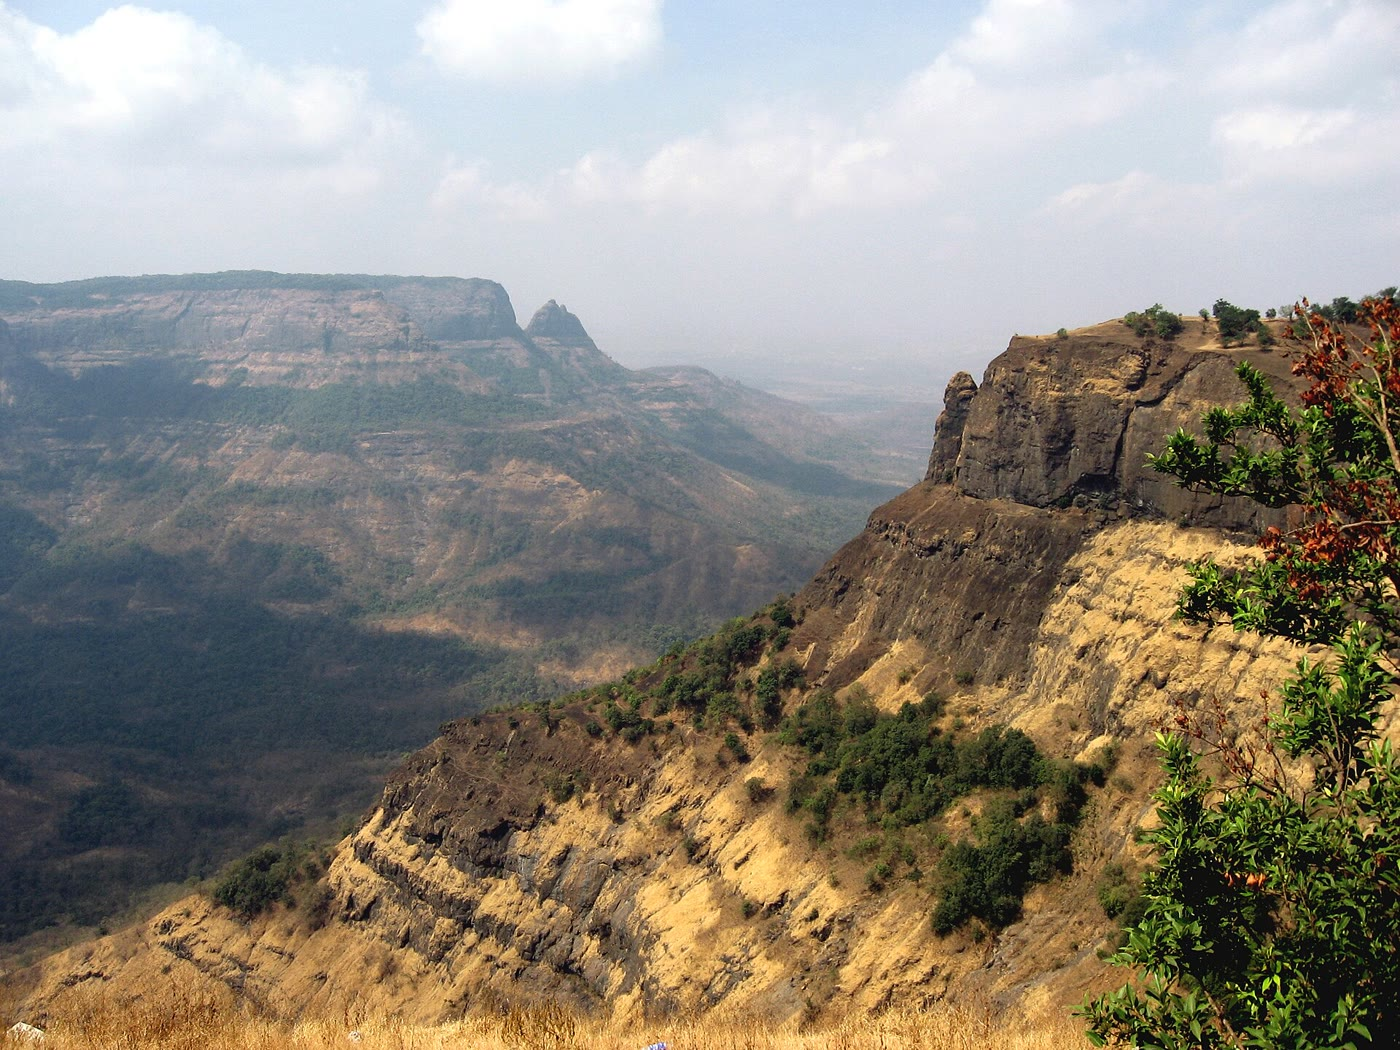
\includegraphics[width=0.55\linewidth]{images/book3/b1-deccan-matheran.jpg}
\par\smallskip{\small Les Ghats occidentaux près de Matheran, en Inde~: des collines à sommet plat
découpées dans un empilement de coulées de lave presque horizontales des trapps du Deccan,
dont les couches résistantes font les marches des versants. Photographie~: Nicholas
(Nichalp), CC BY-SA 2.5 (Wikimedia Commons).}
\label{fig:b1:hotspots:deccan}
\end{omfigure}
% ledger: commons:matheran

\begin{center}
\small
\begin{tabular}{llll}
\hline
province & âge (Ma) & aire (\unit{Mkm^2}) & premier volume (\unit{Mkm^3})\\
\hline
fleuve Columbia & 16 & 0.2 & 0.2\\
Éthiopie--Yémen & 30 & 0.7 & 1.2\\
Atlantique nord & 61 et 56 & 1.2 & plus de 2\\
Deccan & 65.5 & 0.5 (jadis 1.8) & 2 à 4\\
Ontong Java & 122 et 90 & 2 & 44 (\omterm{def:b1:layered-earth:layers}{croûte} entière)\\
Paraná--Etendeka & 133 & 1.5 (jadis plus de 2) & plus de 2.3\\
Karoo--Ferrar & 183 & 3.1 & plus de 2.5\\
Atlantique central (CAMP) & 201 & jadis jusqu'à 7 & plus de 2\\
Trapps de Sibérie & 250 & 0.4 (jadis plus de 4) & plus de 3\\
Emeishan & 259 & 0.5 (jadis 2 à 5) & plus de 1\\
\hline
\end{tabular}
\par\smallskip{\small Âges moyens~; aires telles qu'elles sont aujourd'hui, et telles que
d'abord émises là où une estimation existe~; volumes de lave tels que d'abord émis, sauf pour
le plateau d'Ontong Java, dont le chiffre compte toute sa \omterm{def:b1:layered-earth:layers}{croûte} épaissie. Données~:
V.~Courtillot et P.~Renne (2003).}
\end{center}
% ledger: cr03:table

\noindent Le modèle de panache esquissé à la \cref{sec:b1:hotspots:plumes} explique à la fois la
taille et la hâte~: une tête de panache large de centaines de kilomètres atteint la base
de la \omterm{def:b1:layered-earth:lithosphere}{lithosphère}, se décomprime et fond, et inonde la surface~; puis la
queue continue de construire une \omterm{def:b1:hotspots:track}{trace de point chaud} ordinaire. Plusieurs provinces sont censées
se trouver à l'extrémité ancienne d'une trace vivante~: les trapps du Deccan et le \omterm{def:b1:hotspots:hotspot}{point chaud} de
la Réunion, Paraná--Etendeka et Tristan da Cunha, reliés par la ride de Walvis,
et les basaltes de la Columbia River et Yellowstone.
% ledger: cr03:deccan (Reunion hot spot, plume-head model), be08:ojmh (Parana-Etendeka-Walvis-Tristan), pm90:track (Columbia River basalts)

Les trapps du Deccan, dans l'ouest du centre de l'Inde, sont un empilement de coulées de lave d'environ
\qty{2500}{m} d'épaisseur, dont au moins \qty{1800}{m} ont été émis il y a environ
65.5 millions d'années, en bien moins d'un million d'années~; aujourd'hui ils couvrent
environ \qty{0.5}{\mega km^2}, peut-être \qty{1.8}{\mega km^2} avant l'érosion. Le
plateau d'Ontong Java, dans le sud-ouest du Pacifique, est le plus grand de tous les
plateaux océaniques~: il couvre quelque \qty{2}{\mega km^2}, et sa \omterm{def:b1:layered-earth:layers}{croûte}, épaisse d'environ
\qty{36}{km}, contient quelque \qty{44}{\mega km^3} de roche ignée. Les
plateaux de Manihiki et de Hikurangi, maintenant très éloignés de lui de part et d'autre d'un plancher océanique
plus jeune, ont pu se former avec lui en un seul plateau. La province magmatique de
l'Atlantique central, émise il y a environ 201 millions d'années quand l'Atlantique commençait à
s'ouvrir, est dispersée aujourd'hui, en laves, dykes et filons-couches, sur quatre continents~:
l'est de l'Amérique du Nord, le nord-est de l'Amérique du Sud, l'Afrique de l'Ouest et
le sud-ouest de l'Europe~; elle a pu couvrir jusqu'à \qty{7}{\mega km^2}.
% ledger: cr03:deccan, cr03:table, cr03:ontong-java, be08:ojmh, cr03:camp


Plusieurs provinces coïncident dans le temps avec les grandes extinctions de masse que
décrit la biologie~: les trapps de Sibérie avec la plus grande de toutes, à la fin du
Permien~; la province de l'Atlantique central avec la fin du Trias~; la
Karoo--Ferrar avec une extinction du Jurassique inférieur~; l'Emeishan avec une
au Permien moyen~; et les trapps du Deccan avec la fin du Crétacé. Les
quatre plus grandes extinctions des 260 derniers millions d'années tombent chacune, aussi près
que les dates permettent de le dire, sur l'une de ces provinces, et un lien de cause est
tenu pour le plus probable. Les mécanismes proposés sont atmosphériques~: des aérosols
sulfatés qui refroidissent le climat pour peu de temps, du dioxyde de carbone qui le réchauffe
bien plus longtemps, et des océans privés d'oxygène. Pour la fin du Crétacé,
les éruptions du Deccan ont commencé avant l'impact de Chicxulub et ont continué après
lui~; une revue des enregistrements de la limite a conclu en 2010 que l'impact
a déclenché l'extinction.
% ledger: cr03:table, cr03:summary, cr03:deccan, schulte:kpg

Tout le volcanisme loin des limites de plaques n'a pas besoin d'un panache. De petits
champs volcaniques se développent là où une plaque est étirée ou fissurée, et les chaînes sans
progression nette des âges peuvent être alimentées depuis le \omterm{def:b1:layered-earth:layers}{manteau} supérieur~; c'est l'hypothèse des
plaques à l'œuvre. Ce que deviennent les îles océaniques après le départ du \omterm{def:b1:hotspots:hotspot}{point chaud},
quand elles s'enfoncent, s'usent et font pousser des récifs, relève du volume de deuxième année.
% ledger: fn03:plate-hypothesis

\section{Exercices}

\begin{exercise}[$\star$]\label{exo:b1:hotspots:1}
(a) Le Mauna Kea s'élève à \qty{4205}{m} au-dessus du niveau de la mer, et le fond marin loin de
la chaîne hawaïenne se trouve à \qty{5274}{m} de profondeur. À quelle hauteur le volcan se dresse-t-il
au-dessus de ce plancher~? Pourquoi sa vraie hauteur depuis sa base est-elle plus grande encore~?
(b) Le Mauna Loa contient environ \qty{74000}{km^3}. Combien de temps faudrait-il pour le construire
à l'apport actuel du Kilauea, \qty{0.1}{km^3} par an, et au rythme moyen de
toute la chaîne, \qty{0.025}{km^3} par an~? (c) L'éruption de Pu\textquoteleft
u~\textquoteleft O\textquoteleft o a déversé environ \qty{0.12}{km^3}
par an de 1983 à 2002. Quel volume cela fait-il, et quelle fraction du Mauna Loa~?
% ledger: pp1801:volumes, pp1801:kilauea-supply, pp1801:chain-volume, pp1801:kilauea-rate; 5274 m from hotspots.py
\end{exercise}

\begin{exercise}[$\star$]\label{exo:b1:hotspots:2}
Une plaque tourne au-dessus des \omterm{def:b1:hotspots:hotspot}{points chauds} à \qty{0.92}{\degree\per\Ma}. Prendre
$R = \qty{6371}{km}$. (a) Exprimer $\omega$ en radians par million d'années. (b)
Calculer la vitesse, en \unit{mm.an^{-1}}, de \omterm{def:b1:hotspots:hotspot}{points chauds} à \ang{30}, \ang{60},
\ang{90} et \ang{108.0} du pôle. (c) Pourquoi la vitesse d'Hawaï, à
\ang{108.0}, est-elle inférieure à celle à \ang{90}~?
\end{exercise}

\begin{exercise}[$\star$]\label{exo:b1:hotspots:3}
(a) Calculer l'épaisseur moyenne des trapps du Deccan tels qu'ils sont aujourd'hui,
\qty{1}{\mega km^3} sur \qty{0.5}{\mega km^2}, et de la province de l'Atlantique
central, \qty{2}{\mega km^3} sur \qty{7}{\mega km^2}. (b) Comparer à
l'épaisseur de la coupe du Deccan, \qty{2500}{m}. (c) Pourquoi l'épaisseur moyenne
de la province de l'Atlantique central dit-elle peu de chose de l'épaisseur de
ses empilements de lave~?
% ledger: cr03:table, cr03:deccan, cr03:camp
\end{exercise}

\begin{exercise}[$\star$]\label{exo:b1:hotspots:4}
Une roche de panache plus chaude de \qty{250}{K} que le \omterm{def:b1:layered-earth:layers}{manteau} qui l'entoure a
$\alpha = \qty{3.2e-5}{K^{-1}}$ et $\rho_m = \qty{3300}{kg.m^{-3}}$. (a) De combien
est-elle plus légère, en \unit{kg.m^{-3}}~? (b) Quelle épaisseur d'une telle roche,
étalée sous la plaque, soutiendrait isostatiquement un renflement haut de \qty{690}{m}
sous la mer ($\rho_w = \qty{1000}{kg.m^{-3}}$)~?
% ledger: herzberg:tp (200-300 K), parsons:plate-model (alpha)
\end{exercise}

\begin{exercise}[$\star\star$]\label{exo:b1:hotspots:5}
Deux \omterm{def:b1:hotspots:hotspot}{points chauds} se trouvent sur l'équateur, A à \ang{0}\,E et B à \ang{90}\,E, et
les deux traces vont plein ouest (\omterm{def:b1:spherical-astronomy:horizontal}{azimut} \ang{270}). (a) Calculer les vecteurs de trace
$\vec t_A$ et $\vec t_B$. (b) Calculer $\vec t_A\times\vec t_B$. (c) Appliquer la
règle de signe de la \cref{prop:b1:hotspots:two-tracks}~: où est le \omterm{def:b1:plate-kinematics:euler-pole}{pôle d'Euler}~?
Expliquer le résultat sans calcul. (d) Si A se déplace à \qty{50}{mm.an^{-1}},
quelle est $\omega$ en degrés par million d'années~?
\end{exercise}

\begin{exercise}[$\star\star$]\label{exo:b1:hotspots:6}
Trois \omterm{def:b1:hotspots:hotspot}{points chauds} d'une même plaque se trouvent aux distances $x = R\sin\Delta = 3000$, 5000
et \qty{6000}{km} de l'axe de rotation et se déplacent à 30, 48 et
\qty{57}{mm.an^{-1}}. (a) Ajuster $v = \omega x$ par les moindres carrés et donner
$\omega$ en radians et en degrés par million d'années. (b) Calculer les
résidus. (c) Pourquoi la droite doit-elle passer par l'origine~?
\end{exercise}

\begin{exercise}[$\star\star$]\label{exo:b1:hotspots:7}
Un renflement de section \qty{3e8}{m^2} entoure une \omterm{def:b1:hotspots:track}{trace de point chaud} sur une plaque
se déplaçant à \qty{50}{mm.an^{-1}}. Prendre $\rho_m - \rho_w = \qty{2300}{kg.m^{-3}}$,
$c_p = \qty{910}{J.kg^{-1}.K^{-1}}$ et $\alpha = \qty{3.2e-5}{K^{-1}}$. (a)
Calculer son flux de flottabilité et son flux de chaleur. (b) Comparer avec Hawaï,
\qty{3240}{kg.s^{-1}}. (c) Deux \omterm{def:b1:hotspots:hotspot}{points chauds} ont le même renflement~; l'un se trouve sous une
plaque qui se déplace deux fois plus vite. Quel panache est le plus fort~?
\end{exercise}

\begin{exercise}[$\star\star$]\label{exo:b1:hotspots:8}
Le long de la trace de Yellowstone, les éruptions de caldeiras ont commencé dans le champ
volcanique de McDermitt il y a 16.1 millions d'années et dans le champ de Picabo, à quelque
\qty{350}{km} au nord-est, il y a 10.3 millions d'années~; depuis lors elles se sont
déplacées à $\qty[uncertainty-mode=separate]{2.9 \pm 0.5}{cm}$ par an vers
N\,\ang{54}\,E. (a) À quelle vitesse moyenne le volcanisme a-t-il migré de McDermitt
à Picabo~? (b) Comparer les deux vitesses à celle de la plaque au-dessus du \omterm{def:b1:hotspots:hotspot}{point chaud},
\qty[uncertainty-mode=separate]{26 \pm 5}{mm.an^{-1}} vers \ang{235}. (c) La
direction de la jeune trace est-elle celle attendue~? (d) La partie plus ancienne de la
trace se trouve dans une région qui a été étirée au passage du volcanisme. Comment
cela peut-il expliquer la différence~?
% ledger: pm90:track, data:b3-hotspots
\end{exercise}

\begin{exercise}[$\star\star$]\label{exo:b1:hotspots:9}
Le panache hawaïen porte environ \qty{9.2e10}{W} de chaleur excédentaire. (a) Si tout
s'échappait par les \qty{1000}{km} sur \qty{1000}{km} de fond marin les plus proches du
\omterm{def:b1:hotspots:hotspot}{point chaud}, de combien le flux de chaleur y serait-il augmenté~? (b) Comparer avec
l'excès observé, au plus 5 à \qty{10}{mW.m^{-2}}. (c) Combien de temps la chaleur met-elle à
diffuser à travers une plaque de \qty{100}{km} d'épaisseur ($\kappa = \qty{e-6}{m^2.s^{-1}}$)~?
Combien de temps la plaque met-elle à parcourir \qty{1000}{km} à \qty{92}{mm.an^{-1}}~?
Conclure.
% ledger: vh89:swell-heat
\end{exercise}

\begin{exercise}[$\star\star\star$]\label{exo:b1:hotspots:10}
Les trapps du Deccan contiennent environ \qty{e6}{km^3} de lave. Supposons qu'elle provienne
d'une tête de panache sphérique dont un dixième a fondu. (a) Quels étaient le volume et
le rayon de la tête~? (b) Aplatie sous la \omterm{def:b1:layered-earth:lithosphere}{lithosphère} en un disque épais de
\qty{100}{km}, quel diamètre la tête aurait-elle~? Comparer son aire avec
l'aire que les trapps ont pu couvrir autrefois, \qty{1.8}{\mega km^2}. (c) Si la
lave a été émise en un million d'années, comparer son débit avec l'apport actuel
du Kilauea, \qty{0.1}{km^3} par an. (d) Pourquoi une tête de panache doit-elle être grande,
alors que la queue qui suit est étroite~?
% ledger: cr03:table, pp1801:kilauea-supply
\end{exercise}

\begin{exercise}[$\star\star\star$]\label{exo:b1:hotspots:11}
Entre 81 et 47 millions d'années, le \omterm{def:b1:hotspots:hotspot}{point chaud} hawaïen s'est déplacé vers le sud à plus
de \qty{40}{mm.an^{-1}}. (a) En prenant \qty{40}{mm.an^{-1}}, de quelle distance
s'est-il déplacé~?
(b) Supposons que la plaque se soit déplacée entre-temps à \qty{80}{mm.an^{-1}} vers
\ang{340} au-dessus du \omterm{def:b1:layered-earth:layers}{manteau} profond. Avec $x$ vers l'est et $y$ vers le nord, calculer la
vitesse de la plaque par rapport au \omterm{def:b1:hotspots:hotspot}{point chaud} en dérive, sa vitesse et son
\omterm{def:b1:spherical-astronomy:horizontal}{azimut}. (c) De quel pourcentage, et de combien de degrés, une trace construite
alors déformerait-elle le mouvement de la plaque au-dessus du \omterm{def:b1:layered-earth:layers}{manteau} profond~?
% ledger: tarduno:emperor
\end{exercise}

\begin{exercise}[$\star\star\star$]\label{exo:b1:hotspots:12}
(a) Un basalte de trapps de \qty{e6}{km^3} se refroidit d'environ \qty{1300}{\celsius} à
la température de la surface. Avec une capacité thermique de \qty{3}{MJ.m^{-3}.K^{-1}},
combien de chaleur dégage-t-il (en ignorant la chaleur latente de cristallisation)~?
(b) Étalée sur un million d'années, quelle puissance cela fait-il~? Comparer avec le
panache hawaïen, \qty{9.2e10}{W}, et avec les \qty{47}{TW} de la Terre entière.
(c) Une tête de panache chauffe aussi la base de la \omterm{def:b1:layered-earth:lithosphere}{lithosphère} sans la faire fondre tout
entière. La puissance de (b) est-elle une borne supérieure ou inférieure de la chaleur apportée par la
tête~?
% ledger: delaney86:properties (Book 2 row, 2-3 MJ/m3/K), dd10:total; 1300 degC is an exercise value
\end{exercise}

\section{Problème~: Le compteur de vitesse de la plaque pacifique}

\begin{problem}[{Problème du week-end --- le pôle d'Euler de la plaque pacifique à partir de deux
traces de points chauds, sa vitesse à partir d'une troisième mesure, un test sur d'autres points chauds,
et la flottabilité et l'apport du panache hawaïen}]
\label{pb:b1:hotspots:1}
% values: calc/ch15.py; ledger: data:b3-hotspots, data:etopo1, pp1801:kilauea-supply, pp1801:volumes,
% pp1801:chain-volume, delaney86:properties, parsons:plate-model, dd10:total, data:pb2002 (ridge_budget.py), cd87:rate
Morgan et Morgan listent le \omterm{def:b1:hotspots:hotspot}{point chaud} d'Hawaï à \ang{19.0}\,N, \ang{155.2}\,O,
avec une trace vers $\ang{304}\pm\ang{3}$ et une vitesse de
\qty[uncertainty-mode=separate]{92 \pm 3}{mm.an^{-1}}, et le \omterm{def:b1:hotspots:hotspot}{point chaud} de Louisville
à \ang{53.6}\,S, \ang{140.6}\,O, avec une trace vers $\ang{316}\pm\ang{5}$
et une vitesse de \qty[uncertainty-mode=separate]{67 \pm 5}{mm.an^{-1}}. Utiliser les
axes et les vecteurs $\vec e$, $\vec n$, $\vec t$ de la
\cref{sec:b1:hotspots:tracks}, avec $R = \qty{6371}{km}$. Donner les composantes à
quatre décimales.

\medskip
\noindent\textbf{Partie I --- Le pôle à partir de deux traces.}
\begin{enumerate}
  \item Calculer $\vec r$, $\vec e$ et $\vec n$ à Hawaï, puis le vecteur de
        trace $\vec t_H$.
  \item Faire de même à Louisville~: $\vec r_L$, $\vec e$, $\vec n$ et
        $\vec t_L$.
  \item Vérifier que $\vec t_H$ est un vecteur unitaire perpendiculaire à $\vec r_H$.
  \item Calculer $\vec t_H\times\vec t_L$ et sa longueur. Quel angle font les deux
        vecteurs de trace~?
  \item Normaliser le produit vectoriel et appliquer la règle de signe de la
        \cref{prop:b1:hotspots:two-tracks}.
  \item Donner la \omterm{def:b1:spherical-astronomy:geographic}{latitude} et la \omterm{def:b1:spherical-astronomy:geographic}{longitude} du \omterm{def:b1:plate-kinematics:euler-pole}{pôle d'Euler} de la plaque pacifique
        par rapport aux \omterm{def:b1:hotspots:hotspot}{points chauds}.
\end{enumerate}

\medskip
\noindent\textbf{Partie II --- La vitesse.}
\begin{enumerate}[resume]
  \item Calculer les distances angulaires $\Delta_H$ et $\Delta_L$ du pôle
        aux deux \omterm{def:b1:hotspots:hotspot}{points chauds}.
  \item Calculer $(\vec p\times\vec r_L)\cdot\vec t_L$. Expliquer pourquoi il vaut
        $\sin\Delta_L$, et ce que son signe dit du mouvement à Louisville.
  \item À partir de la vitesse à Louisville, calculer $\omega$ en radians et en
        degrés par million d'années.
  \item Combien de temps la plaque pacifique met-elle à faire un tour complet autour de ce
        pôle~?
  \item Le pôle des moindres carrés des quinze traces du Pacifique se trouve à
        \ang{63.78}\,S, \ang{112.48}\,E, avec \qty{0.92}{\degree\per\Ma}.
        Calculer l'angle entre les deux pôles et comparer les deux vitesses.
\end{enumerate}

\medskip
\noindent\textbf{Partie III --- Un test sur trois autres points chauds.} Morgan et
Morgan donnent le \omterm{def:b1:hotspots:hotspot}{point chaud} de la Société (\ang{18.2}\,S, \ang{148.4}\,O)
\qty[uncertainty-mode=separate]{109 \pm 10}{mm.an^{-1}}, Pitcairn
(\ang{25.4}\,S, \ang{129.3}\,O)
\qty[uncertainty-mode=separate]{90 \pm 15}{mm.an^{-1}} et Cobb
(\ang{46.0}\,N, \ang{130.1}\,O)
\qty[uncertainty-mode=separate]{43 \pm 3}{mm.an^{-1}}.
\begin{enumerate}[resume]
  \item Calculer la distance angulaire du pôle de la question 6 à chacun des
        trois \omterm{def:b1:hotspots:hotspot}{points chauds}.
  \item Prédire les trois vitesses avec la vitesse de la question 9.
  \item Quelles prédictions concordent avec les vitesses mesurées dans leurs
        incertitudes, et lesquelles non~?
  \item Deux traces de directions différentes donnent toujours un pôle. Pourquoi deux
        traces presque parallèles sont-elles un mauvais choix~?
\end{enumerate}

\medskip
\noindent\textbf{Partie IV --- Le panache et le compteur de vitesse.} Le renflement hawaïen
a la section \qty{4.83e8}{m^2}. Prendre
$\rho_m - \rho_w = \qty{2300}{kg.m^{-3}}$, $c_p = \qty{910}{J.kg^{-1}.K^{-1}}$
et $\alpha = \qty{3.2e-5}{K^{-1}}$.
\begin{enumerate}[resume]
  \item Convertir \qty{92}{mm.an^{-1}} en \unit{m.s^{-1}} et calculer le
        flux de flottabilité du panache hawaïen.
  \item Calculer la chaleur excédentaire qu'il porte, et comparer avec les \qty{47}{TW}
        qui quittent la Terre.
  \item Les dorsales font environ \qty{21}{km^3} de \omterm{def:b1:layered-earth:layers}{croûte} par an sur quelque
        \qty{67000}{km}. Quelle longueur de dorsale fait autant de \omterm{def:b1:layered-earth:layers}{croûte} que celle dont
        le Kilauea est alimenté, \qty{0.1}{km^3} par an~?
  \item À ce rythme, combien de temps le Mauna Loa, environ \qty{74000}{km^3},
        mettrait-il à croître~?
  \item Le \omterm{def:b1:hotspots:hotspot}{point chaud} a construit environ \qty{2e6}{km^3} de la chaîne en 81 millions
        d'années. Calculer sa production moyenne et la comparer à l'apport du Kilauea aujourd'hui.
  \item Avec le pôle et la vitesse des parties I et II, calculer la vitesse que
        la trace de Louisville prédit pour la plaque pacifique au-dessus du \omterm{def:b1:hotspots:hotspot}{point chaud}
        hawaïen.
  \item Comparer avec la valeur mesurée \qty[uncertainty-mode=separate]{92 \pm 3}{mm.an^{-1}}~: de combien, et
        de combien d'incertitudes-types, diffèrent-elles~?
  \item À partir des âges des volcans hawaïens, le livre~2 a trouvé \qty{9.1}{cm} par
        an, et les auteurs des âges, en ajustant toute la chaîne,
        \qty{8.6}{cm} par an. Comparer ces moyennes sur des dizaines de millions
        d'années avec les deux vitesses de \omterm{def:b1:hotspots:hotspot}{points chauds}.
  \item À une décimale, en centimètres par an, quelle vitesse la trace de Louisville
        donne-t-elle à la plaque pacifique au-dessus du \omterm{def:b1:hotspots:hotspot}{point chaud} hawaïen~?
\end{enumerate}
\end{problem}
